\documentclass{article}

\usepackage{listings}
\usepackage{xcolor}
\usepackage{indentfirst}
\usepackage{graphicx}

%New colors defined below
\definecolor{codegreen}{rgb}{0,0.6,0}
\definecolor{codegray}{rgb}{0.5,0.5,0.5}
\definecolor{codepurple}{rgb}{0.58,0,0.82}
\definecolor{backcolour}{rgb}{0.95,0.95,0.92}

%Code listing style named "mystyle"
\lstdefinestyle{mystyle}{
	backgroundcolor=\color{backcolour},   commentstyle=\color{codegreen},
	keywordstyle=\color{magenta},
	numberstyle=\tiny\color{codegray},
	stringstyle=\color{codepurple},
	basicstyle=\ttfamily\footnotesize,
	breakatwhitespace=false,         
	breaklines=true,                 
	captionpos=b,                    
	keepspaces=true,                 
	numbers=left,                    
	numbersep=5pt,                  
	showspaces=false,                
	showstringspaces=false,
	showtabs=false,                  
	tabsize=2
}

%"mystyle" code listing set
\lstset{style=mystyle}

\title{Sort clusters algorithms}


\begin{document}
	\maketitle
	\today
	\section{Introduction}
	
	Something about CAL language and a whole BaltiLSC system and the project basic information ...
	
	\section{Data structures}
	\subsection{Cluster-based structures}
	\begin{lstlisting}[language=Python]
	class Resources:
		MEMORY: float # [GB]
		vCPU: int # [quantity of virtual CPU's]
	\end{lstlisting}
	
	The sorting algorithm assume that every virtual Central Process Unit (vCPU) is equal in terms of computation speed. This is a significant generalization becuase actual CPU can have different clock speeds (most of them have 2-3 GHz, but it could have even more than 8 GHz\cite{max_clock_speed}), have different manufacturer and different specification.
	
	\begin{lstlisting}[language=Python,label={lst:Machine}, caption=Machine data structure]]
	class Machine:
		RESOURCES: resources
		PRICE: float # [EURO/h]
	\end{lstlisting}
	
	\begin{lstlisting}[language=Python]
	class Storage:
		SIZE_RANGE: Tuple[float, float] # [GB]
		TYPE: Enum["SSD", "HDD"]
		PRICE: float # [EURO/(TB*h)]
		PricePerHour: float
	\end{lstlisting}
	
	\begin{lstlisting}[language=Python,label={lst:Cluster}, caption=Cluster data structure]]
	class Cluster:
		ID: int
		MACHINES: Dict[str: Machine]
	\end{lstlisting}
	
	\subsection{Application-based structures}
	\begin{lstlisting}[language=Python]
	class Data:
		TYPE: Enum['SET_OF_IMAGES', 'CSV_FILE', ...]
	\end{lstlisting}
	
	\begin{lstlisting}[language=Python]
	class DataSpec(Data):
		QUANTITY: int # The number of data parts, if it is a film it should be 1, if it is a set of photos, it should be the number of photos
		SIZES: [float] # size of each data part [GB]
	\end{lstlisting}
	
	\begin{lstlisting}[language=Python,label={lst:Module}, caption=Module data structure]
	class Module:
		NAME: str
		REQUIRED_RESOURCES: Resources
		INPUT_DATA: Data
	\end{lstlisting}
	
	\begin{lstlisting}[language=Python]
	class JobBatch:
		CLUSTER_ID: int
		MODULES: Dict[str: Module]
		INPUT_DATA: Data
		OUTPUT_DATA: Data
		CAL_DIAGRAM: str # CAL diagram in .yaml format
	\end{lstlisting}
	
	\begin{lstlisting}[language=Python]
	class Task:
		JOB_BATCHES: List[JobBatch]
		INPUT_DATA: DataSpec
		RESOURCES_RESERVATION_RANGE: Tuple[Resources, Rersources]
	\end{lstlisting}
	
	\begin{lstlisting}[language=Python,label={lst:TaskExecution}, caption=TaskExecution data structure]
	class TaskExecutionTime:
		TASK_ID: int
		TIME: float # [s]
	\end{lstlisting}
	
	\begin{lstlisting}[language=Python,label={lst:ModuleSpec}, caption=ModuleSpec data structure]
	class ModuleSpec:
		MODULE_ID: int
		INPUT_DATA: DataSpec
	\end{lstlisting}
	
	\begin{lstlisting}[language=Python,label={lst:ModuleExecutionTime}, caption=ModuleExecutionTime data structure]
	class ModuleExecutionTime:
		MODULE_SPEC_ID: int
		MACHINE: Machine
		TIME: float # [s]
	\end{lstlisting}
	
	\section{Algorithm implemetation}
	\subsection{Input and output data}
	In this subsection we will describe an input and output data for the sorting algorithm. Moreover, we will provide an example input data that will be used to make the algorithm description more clear. 
	
	As a input data for the algorithm we will use:
	\begin{enumerate}
		\item \textit{film\_processor\_job\_batch} (Fig.~\ref{job_batch_example}): JobBatch - the job batch that we want to execute,
		\item \textit{matching\_clusters}: List[Cluster] - list of clusters that meet resources reservation range of the \textit{film\_processor\_job\_batch}
		\item \textit{time\_price\_ratio}: float [0,1] - the priority of sorting policy set up by user who is executing the task
	\end{enumerate}

	As a output data of the algorithm we receive a list of sorted clusters with list of a pairs Module to Machine for each cluster. Additionaly we receive the instruction (configuration) of how to run each module (the internal modules parralelization) and when (parallelization between modules). You can find more about modules parralelization in the algorithm scheme indtroduced further. 
	
	If there are appropriate data, the algorithm besides, it sorts clusters, predict the execution time of a job batch. Otherwise, we just receive the relative (not real) executions times. The same situation we have with overall price. We should provide specific data to receive the real price estimation. The example output can look like this (Machine, Cluster and Module simplified data structures are shown in listening~\ref{lst:Machine},~\ref{lst:Cluster} and ~\ref{lst:Module}):
	
	\begin{lstlisting}[language=Python,label={lst:AlgorithmOutput}, caption=Example output of the sorting algorithm]
	[
		(
			c_1: Cluster, 
			[ # These are the module to machine bindings with modules parralelization configuration
				(m_1: Module, M_1: Machine, n: float, block: float),
				(m_2: Module, M_1: Machine, n: float, block: float),
				(m_3: Module, M_4: Machine, n: float, block: float),
				...
			],
			overall_time: float,
			is_time_real: bool,
			overall_price: float,
			is_price_real: bool,
		),
		(
			...
		),
		...
	]
	\end{lstlisting}
	
	\subsection{Algorithms utils}
	
	Let's get through our algorithms with a job batch as follows:
	
	\begin{figure}[h]
		\caption{\textit{film\_processor\_job\_batch} implementation with CAL language}
		\label{job_batch_example}
		\centering
		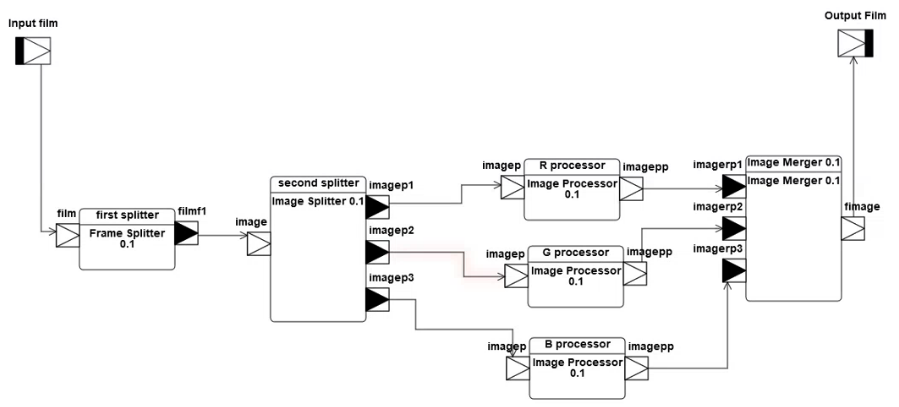
\includegraphics[width=1\textwidth]{example_app}
	\end{figure}
	
	\begin{lstlisting}[language=Python]
	film_processor_job_batch = JobBatch(
		MODULES = {
			'first splitter': m1,
			'second splittter': m2,
			'R processor': m3,
			'G processor': m3,
			'B processor': m3,
			'Image Merger 0.1': m4,
		},
		INPUT_DATA = Data(
			TYPE = 'FILM'
		),
		OUTPUT_DATA = Data(
			TYPE = 'FILM'
		),
		CAL_DIAGRAM = '(call diagram content based on application implementation)',
	)
	\end{lstlisting}
	
	An example Task structure is listen below:
	\begin{lstlisting}[language=Python]
	film_processor_task = Task(
		JOB_BATCHES = [film_processor_job_batch],
		INPUT_DATA: DataSpec(film_processor_job_batch.INPUT_DATA) (
			QUANTITY = 1
			SIZES = [1.2]
		),
		RESOURCES_RESERVATION_RANGE: (
			Resources(
				vCPU = 1,
				MEMORY = 1,
			), 
			Rersources(
				vCPU = 32,
				MEMORY = 32,
			)
		)
	)
	\end{lstlisting}
	
	Let's assume that we have for a disposition the following clusters:
	\begin{itemize}
		\item \textit{gcp\_cluster}\cite{gcp_cluster}
		\item \textit{aws\_cluster}\cite{aws_cluster}
		\item \textit{tartu\_cluster}\cite{tartu_cluster}
	\end{itemize}
	In the listening below we can find details for each cluster (this are the original machines and prices from the given providers, limited to the most popular machines for the sake of simplicity in explaining the sorting algorithm):
	
	\begin{lstlisting}[language=Python]
	gcp_cluster: Cluster = Cluster(
		ID: 1,
		MACHINES: {
			'e2-standard-2': Machine = (
				RESOURCES: {
					MEMORY = 8
					vCPU = 2
				}
				PRICE = 0.067
			),
			'e2-standard-4': Machine = (
				RESOURCES: {
					MEMORY = 16
					vCPU = 4
				}
				PRICE = 0.13
			),
			'e2-highcpu-8': Machine = (
				RESOURCES: {
					MEMORY = 8
					vCPU = 8
				}
				PRICE = 0.20
			)
		},
	),
	aws_cluster: Cluster = Cluster(
		ID: 2,
		MACHINES: {
			'm5.large': Machine = (
				RESOURCES: {
					MEMORY = 2
					vCPU = 4
				},
				PRICE = 0.135 
			),
			'm5.xlarge': Machine = (
				RESOURCES: {
					MEMORY = 4
					vCPU = 16
				},
				PRICE = 0.23 
			),
			'r5.xlarge': Machine = (
				RESOURCES: {
					MEMORY = 4
					vCPU = 32
				},
				PRICE = 0.304
			)
		},
	),
	tartu_cluster: Cluster = Cluster(
		ID: 3,
		MACHINES: {
			'small': Machine = (
				RESOURCES: {
					MEMORY = 6
					vCPU = 1
				},
				PRICE = 0.014
			),
			'megium': Machine = (
				RESOURCES: {
					MEMORY = 6
					vCPU = 4
				},
				PRICE = 0.064
			),
			'large': Machine = (
				RESOURCES: {
					MEMORY = 16
					vCPU = 8
				},
				PRICE = 0.112
			),
		},
	)
	\end{lstlisting}
	

	\subsection{Algorithm scheme}
	Let's indtroduce the following assumptions:
	
	\begin{enumerate}
		\item Each instance of any vCPU is equal in terms of computation speed, regardless of the cluster it belongs to.
		\item The output is a list of sorted clusters with  task execution details (parralelization configuration).
		\item Algorithm estimates the relative (in relation to other clusters) costs and times of task execution. It can provide real time and price estimation but the appropriate amount of specific historical data is required.
	\end{enumerate}  

	Algorithm consist of the following steps:
	
	\begin{enumerate}
		\item Construct the modules data specifications. Running the JobBatch, we have only the specification of input data for the first module. Subsequent modules take the data from the previous ones and we can use any method to predict  (or establish from the module specification) the output data specification. In our example we assume that all of the data specifications have the same size and quantity (the size and quantity of the JobBatch input data) or the quantity and size will be reduce based on input data type of specific module.
		\begin{lstlisting}[language=Python]
		>>> getModulesDataSpec(film_processor_job_batch)
		[
			'first_splitter': DataSpec(m1.INPUT_DATA) (
				QUANTITY = 1,
				SIZES = [1.2],
			),
			'second_splitter': DataSpec(m2.INPUT_DATA) (
				QUANTITY = 1,
				SIZES = [1.2],
			),
			'R processor': DataSpec(m3.INPUT_DATA) (
				QUANTITY = 1,
				SIZES = [1.2],
			),
			'G processor': DataSpec(m3.INPUT_DATA) (
				QUANTITY = 1,
				SIZES = [1.2],
			),
			'B processor': DataSpec(m3.INPUT_DATA) (
				QUANTITY = 1,
				SIZES = [1.2],
			),
			'Image Merger 0.1': DataSpec(m4.INPUT_DATA) (
				QUANTITY = 1,
				SIZES = [1.2],
			),
		]
		\end{lstlisting}
		\item Return the list of module to machine pairs (with probabilities of each matching) for each cluster. It takes into the consideration resource reservation range and resources requirements for each module. The probability can depends on how fequently the modules are assigned to each machine (the extended version of the algorithm using historical data). In this simple example we assume uniform distribution of probabilities. The function takes into the consideration only the machines from clusters for which resources are in the Task resources reservation range. In our example all of the machines at all of clusters are in the resources reservatuin range for the \textit{film\_processor\_job\_batch}.
		
		
		\begin{lstlisting}[language=Python]
		{
			1: [
				(m1, [
						('e2-standard-2', 1/3),
						('e2-standard-4', 1/3),
						('e2-highcpu-8', 1/3),
					]
				),
				...
				(m6, [
						('e2-standard-2', 1/3),
						('e2-standard-4', 1/3),
						('e2-highcpu-8', 1/3),
					]
				),
				],
				2: [
				(m1, [
						('m5.large', 1/3),
						('m5.xlarge', 1/3),
						('r5.xlarge', 1/3),
					]
				),
				...
				(m6, [
						('m5.large', 1/3),
						('m5.xlarge', 1/3),
						('r5.xlarge', 1/3),
					]
				),
				],
				3: [
				(m1, [
						('small', 1/3),
						('medium', 1/3),
						('large', 1/3),
					]
				),
				...
				(m6, [
						('small', 1/3),
						('medium', 1/3),
						('large', 1/3),
					]
				),
			]
		}
		\end{lstlisting}
		
		\item Estimate the module execution time for each of the pairs (module to machine) with no zero propability. The estimation of execution time for each module-to-machine pair is based on historical data of the module executions. For each module we create the simple machine learning model with the execution time as the explained variable and the following features:
		\begin{itemize}
			\item machine CPU resources where the module was executed
			\item data input features like the total size of the input data or the number of elements of the input data set
		\end{itemize}
		As we know the input data and the resources of the machine on which the module will be executed, we can ask our model about the execution time estimation.
		Here we have an example output for the first and the last pair of cluster 1 (we have replaced the machine name with it price to make futher price calculations possible): 
		\begin{lstlisting}[language=Python]
		{
			1: [
					(m1, [
							(0.067, 1/3, 32.54),
							(0.13, 1/3, 28.44),
							(0.20, 1/3, 21.11),
						]
					),
					...
					(m6, [
							(0.067, 1/3, 122.11),
							(0.13, 1/3, 111.47),
							(0.20, 1/3, 91.26),
						]
					)
				],
			...
		}
		\end{lstlisting}
		\item*\footnote{Steps marked with * sign are the additional steps to provide the better estimations of execution time and price but are not necessary to perform clusters sorting.} If we have enough computational power assured by the resources reservation range and the module can be run in parallel it can decrease the execution time by \textit{n} times, where \textit{n} is the amount of machine instances executing the module. Figure~\ref{fig:timeline} shows the example internal modules parallelization with \textit{n} equal to 1, 3, 4 and 1 respectively for module 1, 2, 3 and 4.
		
		Moreover, different modules can be executed in the same time if the application specification allows to do that. Let's assume that the \textit{first\_splitter} (which splits film into frames) can be executed part by part in the same time with \textit{second\_splitter} (which takes the image and return the 3 images, one for each RGB channel) and the \textit{R/G/B\_processor} as well. 
		With the assumption described above the \textit{film\_processing\_task}`s execution time line can look like it is shown on the figure~\ref{fig:timeline_2}.
		
		Since we estimated the execution times for each module in the previous step, now we can find all possible parallelization configuration for the job batch and further search for the best one.
		
		In our example we simplify this step by providing only the single one configuration where there is no any parallelization at all:
		\begin{lstlisting}[language=Python]
		{
			1: [
			"c1_conf1": [
					(m1, [
							(0.067, 1/3, 32.54),
							(0.13, 1/3, 28.44),
							(0.20, 1/3, 21.11),
						], 1, 0
					),
					...
					(m6, [
						(0.067, 1/3, 122.11),
						(0.13, 1/3, 111.47),
						(0.20, 1/3, 91.26),
						], 1, 5
					)
				],
			],
			...
		}
		\end{lstlisting}
		The last part of each module element for a given configuration tell us which modules can be executed in the same time. One part before last is the \textit{n} factor (which in our example is equal to 1 everywhere) and it will be used further to divide the modules execution time estimations and also provide information about the way of a task execution.
		\item* As we can see on the Figure~\ref{fig:timeline} there could be some time windows between modules executions. This windows represents the time to start the instance of machine and other preparations before module execution like start up the image or download the data. This step is sophisticated and it should not provide a large changes to final result but if we would like to have better estimations it should be carry out. It could be done by:
		
		\begin{itemize}
			\item Intodruce the function that returns internal flow ratio of the JobBatch execution based on input data size and the parallelization configuration. In our example AIRF (\textit{application interfnal flow ratio}) function can look like it is shown on the figure~\ref{fig:aifr}. To be more specific, it returns overall time of task execution minus sum of the maximum executions times of each modules from the task execution time line. The function use the following formula:
			\begin{equation}
			coeff =  \frac{internal\_flow\_time}{task\_execution\_time }
			\end{equation}
			In the example timeline shown on the figure~\ref{fig:timeline} (where modules internal parallization respectively equals 1, 3, 4, 1) the coefficient will eqaul:
			\begin{equation}
			coeff =  \frac{T - t1 - t2 - t3 - t4}{T}
			\end{equation}
			
			So as a result we get the internal flow coefficient (\textit{IFC}) in range [0, 1] the value of which reflects the ratio of internal data flow between modules time and the task execution time. If there is no need for modules to be executed in sequence (one after another), it is possible that later modules will be executed in parallel with the earlier ones. This is shown in Figure~\ref{fig:timeline_2}. In such a case the \textit{IFC} will be significantly lower. Even though, it is possible to count the \textit{IFC} for such a cases taking into the account the task execution configuration. Having the IFC for a task we just multiply each estimated module execution time by factor 1 + \textit{IFC}.
			\item Other approximation of the internal data flow time by looking at the historical data of modules executions.
		\end{itemize}
		\item An user responsible for the task execution is providing \textit{time-price} ratio which is the factor prioritizing the cluster sorting. It is a float number from 0 to 1 telling the algorithm if user is willing to save more time or money.
		
		In this step we count the best parallelization configuration for each cluster based on the \textit{time-price} ratio. For each configuration we aggregate a time and a price for each module receiving the overall time and price of a task execution. Next we normalize the prices and times for each configuration within the cluster and use the \textit{time-price} ratio to find the best one.
		
		The listing below show the aggregation result: 
		\begin{lstlisting}[language=Python]
		{
			1: [
					(m1, (3.33, 27.36), 1, 0),
					...
					(m6, (13,49, 108,28), 1, 5),
				],
			...
		}
		\end{lstlisting}
		In this step we had ready the estimates of execution price and time for each module on each cluster.
	
		\item* It needs to be highlighted that we sort clusters for a JobBatch. JobBatch is a part of a Task and if we consider a Task with a few JobBatches we have to include data transfer time beetwen cluster in the sorting algorithm. It will be realized through introducing the data tranfer time coefficient (\textit{DTTC}). For instance, if a previous JobBatch was executed at Cluster `A`, then actual JobBatch will have the \textit{DTTC} equal to one for Cluster `A` and eqaul to more than one to Cluster `B`. Time-pricing ratios will be multiply by the corresponding \textit{DTTC} and thus we will get the final time-pricing ratios. 
		\textit{DTTC} can be based on historical data of jobs executions that run different batches on different clusters. As this step is enought sophisticated to perform with more complex scenarios, it is omitted by now.
		\item The final step is counting the overall time and price for each cluster and then sort them by using the time-price ratio.
		We got the following overall times and prices with the task execution configurations:
		\begin{lstlisting}[language=Python]
		{
			1: (41.22, 287.17, "c1_conf1"),
			2: (61.81, 221.18, "c2_conf1"),
			3: (51.11, 181.19, "c3_conf1"),
		}
		\end{lstlisting}
		Having the \textit{time-price} ratio eqaul to 0.6 (which means that the user is willing to save time a little more than money) we got the following final penalty for each cluster:
		\begin{lstlisting}[language=Python]
		{
			1: 41.22 * (1-0.6) + 287.17 * 0.6 = 188,79,
			2: 61.81 * 0.4 + 221.18 * 0.6 = 157,42,
			3: 51.11 * 0.4 + 181.19 * 0.6 = 129,16,
		}
		\end{lstlisting}
		
		The smaller penalty is, the more suitable the cluster is for given task execution and \textit{time-price} ratio. The final list of sorted clusters:
		
		\begin{lstlisting}[language=Python]
		[
			(3, 129,16, "c3_conf1"),
			(2, 157,42, "c2_conf1"),
			(1, 188,79, "c1_conf1"),
		]
		\end{lstlisting}
		
		If the probabilities of matching module to machine have uniform distribution (this happen when we do not have historical data of modules executions) and all of the machines resources are in the task resources reservation range, and we do not use any parralelization, the algorithm is just counting the average price of a machine for each cluster and that what the sorting is based on.
		
	\end{enumerate}
	
	\begin{figure}[!htb]
		\caption{Example of the \textit{file\_processor\_task} timeline with internal module parallelization.}
		\label{fig:timeline}
		\centering
		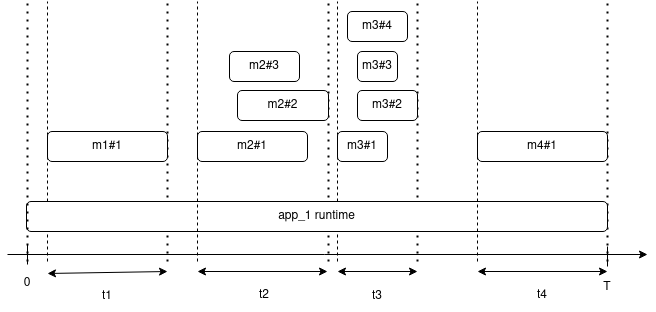
\includegraphics[width=1\textwidth]{timeline}
	\end{figure}
	\begin{figure}[!htb]
		\caption{Example of the \textit{file\_processor\_task} timeline with internal module parallelizations and between modules parallelization as well.}
		\label{fig:timeline_2}
		\centering
		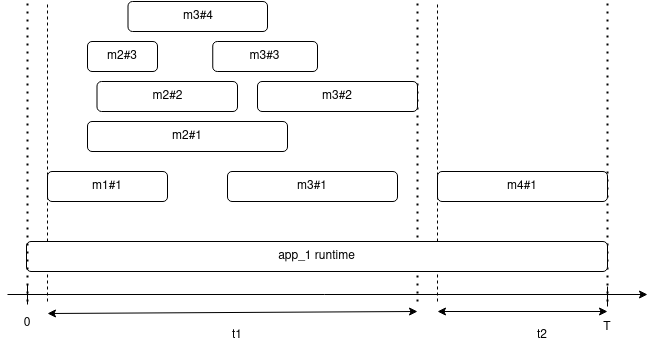
\includegraphics[width=1\textwidth]{timeline_2}
	\end{figure}
	\begin{figure}[h]
		\caption{\textit{file\_processor\_task} \textit{AIFR}}
		\centering
		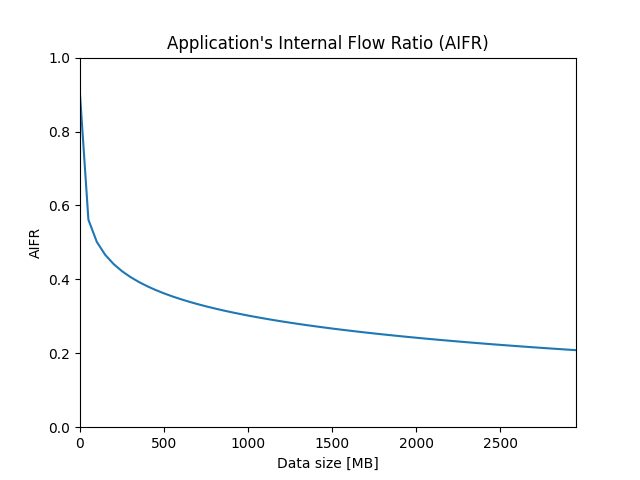
\includegraphics[width=1\textwidth]{AIFR}
		\label{fig:aifr}
	\end{figure}
	\newpage
	
	\section{Algorithms tests}
	\section{Conclusions}
	
	\begin{thebibliography}{9}
		\bibitem{gcp_cluster} 
		Google: Google Clound Platform - pricing, 03.10.2020,
		\\\texttt{https://cloud.google.com/compute/all-pricing}
		\bibitem{max_clock_speed} 
		asus.com: 8.79GHz FX-8350 Is The Fastest Ever CPU, 03.10.2020,
		\\\texttt{https://rog.asus.com/articles/crosshair-motherboards/8-79ghz-fx-8350-is-the-fastest-ever-cpu/}
		\bibitem{aws_cluster}
		Amazon: Amazon Web Services - pricing, 04.10.2020,
		\\\texttt{https://aws.amazon.com/emr/pricing/}
		\bibitem{tartu_cluster}
		University of Tartu, HPC - pricing, 04.10.2020,
		\\\texttt{https://hpc.ut.ee/en/prices/}
	\end{thebibliography}

\end{document}